%% PQ-uArch -- paper skeleton for the Journal of Systems Architecture (Elsevier, elsarticle)
%% SUPERVISOR RULE: no AI-written prose. Every [AUTHOR TO WRITE] block must be written
%% by the author. The "FACTS" lists under each block are notes taken from the results
%% (numbers come from facts.tex, regenerated by make_facts.py). Delete the FACTS lists
%% once the prose is written. Anything marked [CHECK WITH AUTHOR] is unverified.
\documentclass[preprint,12pt,authoryear]{elsarticle}
\usepackage{amsmath,amssymb,booktabs,graphicx,xcolor,hyperref,siunitx,multirow}
\newcommand{\AW}[1]{\par\noindent\colorbox{yellow!40}{\parbox{\linewidth}{\textbf{[AUTHOR TO WRITE]} #1}}\par}
\newcommand{\CK}[1]{\textcolor{red}{[CHECK WITH AUTHOR: #1]}}
\newenvironment{facts}{\par\small\noindent\textbf{FACTS (notes, delete after writing):}\begin{itemize}\setlength\itemsep{0pt}}{\end{itemize}\normalsize}
% generated by make_facts.py -- do not edit by hand
\newcommand{\FactNumBuilds}{81}
\newcommand{\FactKeccakShareKemMin}{36}
\newcommand{\FactKeccakShareKemMax}{55}
\newcommand{\FactKeccakShareDsaMin}{33}
\newcommand{\FactKeccakShareDsaMax}{65}
\newcommand{\FactMulGainKem}{2.24}
\newcommand{\FactBpGainKem}{1.05}
\newcommand{\FactCFourLossKem}{41}
\newcommand{\FactMulGainDsa}{2.01}
\newcommand{\FactBpGainDsa}{1.05}
\newcommand{\FactCFourLossDsa}{49}
\newcommand{\FactCSixteenLoss}{4}
\newcommand{\FactIcMissBaseTwo}{36}
\newcommand{\FactIcMissAllOne}{1.0}
\newcommand{\FactIcNeedBase}{8}
\newcommand{\FactIcNeedAll}{1}
\newcommand{\FactAllSpeedMin}{2.34}
\newcommand{\FactAllSpeedMax}{3.67}
\newcommand{\FactAllSpeedGm}{3.17}
\newcommand{\FactKSpeedMin}{1.48}
\newcommand{\FactKSpeedMax}{2.80}
\newcommand{\FactKSpeedGm}{2.01}
\newcommand{\FactMSpeedMin}{1.07}
\newcommand{\FactMSpeedMax}{1.35}
\newcommand{\FactMSpeedGm}{1.22}
\newcommand{\FactKLsSpeed}{1.73}
\newcommand{\FactAllLsSpeed}{2.54}
\newcommand{\FactGccSlow}{1.45}
\newcommand{\FactGccAllSpeed}{2.71}
\newcommand{\FactPqmRatioMin}{1.25}
\newcommand{\FactPqmRatioMax}{1.28}
\newcommand{\FactKLatFast}{2.02}
\newcommand{\FactKLatSlow}{1.51}
\newcommand{\FactAllAreaPct}{211}
\newcommand{\FactAllLsAreaPct}{115}
\newcommand{\FactLsGE}{12,730}
\newcommand{\FactKfGE}{42,374}
\newcommand{\FactValRuns}{24}
\newcommand{\FactValMaxErr}{0.000}
\newcommand{\FactValAllExact}{yes}
\newcommand{\FactGccDivPrefix}{4688}
\newcommand{\FactGccDivBase}{80}

\journal{Journal of Systems Architecture}

\begin{document}
\begin{frontmatter}
\title{\AW{Title. Suggested direction: performance, ISA extensions and microarchitecture-dependent timing leakage of FIPS 203/204 lattice cryptography on embedded in-order RISC-V pipelines}}
\author[nsu]{Md. Rakib Rayhan\corref{cor}}
\ead{\CK{email}}
\author[nsu]{\CK{co-authors / supervisor order}}
\cortext[cor]{Corresponding author}
\affiliation[nsu]{organization={Microprocessor, Embedded Systems, and IoT Lab (MESIL), Department of Electrical and Computer Engineering, North South University},
  city={Dhaka}, postcode={1229}, country={Bangladesh}}

\begin{abstract}
\AW{Abstract, 150--250 words.}
\begin{facts}
\item Simulator: RV32IM ISS with cycle-level 5-stage in-order timing model; PQClean clean ML-KEM-512/768/1024 and ML-DSA-44/65/87; outputs bit-exact with native builds for all \FactNumBuilds{} builds (clang and gcc).
\item Validation: cycle-exact against the RTL of the author's FPGA-proven RV32IM 5-stage core -- \FactValRuns{} held-out runs (kernels and full ML-KEM/ML-DSA, 2 compilers, 2 multipliers), maximum cycle error \FactValMaxErr\,\%.
\item Keccak-f[1600] is \FactKeccakShareKemMin--\FactKeccakShareKemMax\,\% of ML-KEM cycles on C1-TB5.
\item Multiplier choice: single-cycle vs iterative = \FactMulGainKem$\times$ (ML-KEM), \FactMulGainDsa$\times$ (ML-DSA); branch prediction adds only \FactBpGainKem$\times$.
\item All custom instructions: \FactAllSpeedMin--\FactAllSpeedMax$\times$ speed-up; Keccak instruction alone \FactKSpeedMin--\FactKSpeedMax$\times$.
\item Added area for all units: \FactAllAreaPct\,\% of the baseline core with a one-round-per-cycle Keccak unit; \FactAllLsAreaPct\,\% (+3.2\,kbit RAM) with the lane-serial unit, which keeps \FactAllLsSpeed$\times$ (vs \FactAllSpeedGm$\times$).
\item Base code needs an \FactIcNeedBase\,KB I-cache; with the Keccak instruction \FactIcNeedAll\,KB suffices.
\item Leakage: see Section~\ref{sec:leak} facts.
\end{facts}
\end{abstract}
\begin{keyword}
Post-quantum cryptography \sep ML-KEM \sep ML-DSA \sep RISC-V \sep instruction-set extension \sep timing side channel \sep microarchitecture simulation
\end{keyword}
\end{frontmatter}

%% =====================================================================
\section{Introduction}\label{sec:intro}
\AW{Motivation (quantum threat, FIPS 203/204 published Aug.~2024, migration deadlines), why embedded RV32 in-order cores matter, the three questions this paper answers, contributions list, paper organisation.}
\begin{facts}
\item Contributions to claim (defensible after literature review):
  (C1) FIPS-final clean baselines on a parameterised RV32IM in-order pipeline (not found in published literature);
  (C2) joint microarchitecture DSE (branch predictor, multiplier, divider, caches, RAS) for both ML-KEM and ML-DSA;
  (C3) latency-swept Keccak instruction plus modular-arithmetic/butterfly instructions, with synthesised area;
  (C4) timing leakage measured as a function of individually toggled microarchitecture knobs, holding ISA, compiler and code fixed, including the effect of the ISA extensions on leakage;
  (C5) cycle-exact validation of the timing model against the RTL of a real FPGA-proven RV32IM core (rare for PQC ISE papers, which usually report FPGA cycles without a validated model);
  (C6) compiler study: gcc 13 re-introduces the KyberSlash division from the pre-2024 C source at -O2 and -Os, clang 18 does not;
  (C7) open-source, reproducible framework.
\item Do NOT claim: first ML-KEM/ML-DSA ISE (PQCUARK, HORCRUX, OpenTitan), first Keccak instruction (RISQ-V, Karl et al.), first TVLA across RISC-V cores (Mishra et al.~2026), first division leakage (KyberSlash).
\end{facts}

%% =====================================================================
\section{Background}\label{sec:bg}
\subsection{ML-KEM and ML-DSA}
\AW{Module lattices, NTT, Keccak/SHAKE usage, parameter sets, FO transform with implicit rejection.}
\subsection{Embedded in-order RISC-V pipelines}
\AW{5-stage pipeline (cite Harris \& Harris), hazards, branch resolution, M-extension multiplier/divider options.}
\subsection{Timing side channels from variable-latency hardware}
\AW{Early-terminating multipliers \citep{grossschadl2009}, KyberSlash \citep{kyberslash2025}, constant-time contracts and Zkt \citep{riscvzkt,leave2023}, TVLA/dudect \citep{dudect2017}.}

%% =====================================================================
\section{Related work}\label{sec:related}
\AW{Groups: (i) pre-standard lattice ISEs on RISC-V \citep{alkim2020isa,fritzmann2020risqv,nannipieri2021,karl2023sig,miteloudi2023pqvalue,gewehr2024};
(ii) FIPS-era ISEs and coprocessors \citep{pqcuark2025,horcrux2025,otbn2025};
(iii) software baselines \citep{pqm4,pqclean};
(iv) variable-latency timing channels \citep{grossschadl2009,kyberslash2025,phantom2026};
(v) microarchitecture leakage and contracts \citep{leave2023,mishra2026chips,riscvzkt};
(vi) simulator validation \citep{roelke2017risc5,ta2018gem5}.}
\begin{table}[t]\centering\caption{Positioning against prior work (gap table from the literature review). \AW{caption}}\label{tab:gap}
% from the literature review; verify each cell [CHECK WITH AUTHOR]
\resizebox{\linewidth}{!}{\begin{tabular}{lllllll}\toprule
Work & FIPS 203/204 & KEM+DSA & Target & $\mu$arch DSE & ISE incl.\ Keccak & Timing leakage \\\midrule
Alkim et al. 2020 & -- & -- & RV32 & partial & no Keccak & -- \\
RISQ-V 2020 & -- & -- & RV32 & -- & yes & -- \\
Karl et al. 2023 & -- & DSA only & RV32 & -- & yes & -- \\
PQ.V.ALU.E 2024 & -- & yes & RV32 & partial & no Keccak & -- \\
PQCUARK 2025 & yes & yes & RV64 & -- & yes & -- \\
KyberSlash 2025 & partly & KEM & real HW & -- & -- & fixed platforms \\
Mishra et al. 2026 & -- & -- & RV64 cores & whole cores & -- & yes (not PQC) \\
Phantom 2026 & yes & KEM & one M4 & -- & -- & one core \\
This work & yes & yes & RV32 in-order & yes & yes, latency-swept & per knob, with ISE \\
\bottomrule
\end{tabular}}

\end{table}

%% =====================================================================
\section{The PQ-uArch framework}\label{sec:framework}
\AW{Figure 1 (draw in TikZ/draw.io): PQClean source $\rightarrow$ patcher (ISA variants) $\rightarrow$ clang RV32IM $\rightarrow$ ISS + timing model $\rightarrow$ profiler / DSE / TVLA; native build for cross-check.}
\subsection{Timing model}
\AW{Scoreboard formulation of the 5-stage pipeline; parameters in Table~\ref{tab:params}.}
\begin{facts}
\item One instruction enters EX per cycle; full forwarding; load-use = 1 cycle; branches resolved in EX, mispredict = 2 cycles; JAL = 1 (dynamic-predictor cores) or 2 cycles; RAS optional.
\item Multiplier: iterative 32 cycles (stalls), pipelined 3-cycle, single-cycle, early-terminating on rs2 (ARM7TDMI-style, 8 bits/cycle), early-terminating on the smaller operand. Divider: fixed 34 cycles or early-out (skips leading quotient zeros).
\item Caches: blocking, set-associative, LRU, write-back/write-allocate, 32-byte lines; memory latency 20 cycles in the cache studies.
\item Verified with hand-derived micro-benchmarks (load-use, loops, multiplier, divider): \texttt{step1\_simulator/verify\_timing.py} -- method follows \citep{ta2018gem5}.
\end{facts}
\subsection{PQC instruction-set extensions}
\begin{table}[t]\centering\caption{Custom-0 (opcode 0x0B) instructions. \AW{caption}}\label{tab:isa}
\begin{tabular}{lll}\toprule
Mnemonic & funct3 & Semantics \\\midrule
pq.kmred & 0 & $rd \leftarrow \mathrm{MontRed}_{3329}(rs1)$ \\
pq.kmul & 1 & $rd \leftarrow \mathrm{MontRed}_{3329}(rs1_{[15:0]}\cdot rs2_{[15:0]})$ \\
pq.kbar & 2 & $rd \leftarrow \mathrm{Barrett}_{3329}(rs1_{[15:0]})$ \\
pq.kct / pq.kgs & 3 / 4 & packed 16-bit CT / GS butterfly, $rs2=\zeta$ \\
pq.dmul & 5 & $rd \leftarrow \mathrm{MontRed}_{8380417}(rs1\cdot rs2)$ \\
pq.cmul & 6 & fixed-latency multiply (low / high word by funct7) \\
pq.keccak & 7 & Keccak-f[1600] on the 200-byte state at $[rs1]$ \\\bottomrule
\end{tabular}\end{table}
\subsection{Timing validation against RTL}
\AW{Describe: the author's RV32IM 5-stage core (Harris \& Harris style, synchronous M9K memories, iterative M unit, tested on a Cyclone IV board) simulated with Icarus Verilog; same ELF binaries on PQ-uArch with the matching configuration; calibration then held-out validation.}
\begin{table}[t]\centering\caption{Calibration: cycles per pattern, RTL vs PQ-uArch. Only the M-unit occupancy was fitted. \AW{caption}}\label{tab:calib}
\resizebox{\linewidth}{!}{\begin{tabular}{lrrrrrr}\toprule
 & \multicolumn{3}{c}{serial multiplier} & \multicolumn{3}{c}{embedded multiplier}\\
Pattern & RTL & sim (datasheet) & sim (calibrated) & RTL & sim (datasheet) & sim (calibrated)\\\midrule
ALU (addi) & 1 & 1 & 1 & 1 & 1 & 1 \\
load + dependent use & 3 & 3 & 3 & 3 & 3 & 3 \\
store + load & 2 & 2 & 2 & 2 & 2 & 2 \\
taken branch & 3 & 3 & 3 & 3 & 3 & 3 \\
not-taken branch & 1 & 1 & 1 & 1 & 1 & 1 \\
jal & 3 & 3 & 3 & 3 & 3 & 3 \\
call + return & 9 & 9 & 9 & 9 & 9 & 9 \\
mul & 35 & 34 & 35 & 4 & 3 & 4 \\
mulh & 35 & 34 & 35 & 4 & 3 & 4 \\
mulhu & 35 & 34 & 35 & 4 & 3 & 4 \\
div & 39 & 37 & 39 & 39 & 37 & 39 \\
remu & 39 & 37 & 39 & 39 & 37 & 39 \\
mul + dependent add & 36 & 35 & 36 & 5 & 4 & 5 \\
\bottomrule
\end{tabular}
}\end{table}
\begin{table}[t]\centering\caption{Held-out validation against the RTL core. \AW{caption}}\label{tab:rtlval}
\resizebox{\linewidth}{!}{\begin{tabular}{lllrrrc}\toprule
Kernel & Compiler & Multiplier & RTL cycles & Sim.\ cycles & Error (\%) & Hash match \\\midrule
SHAKE256, 1 KB & clang & serial & 143,221 & 143,221 & 0.000 & yes \\
SHAKE256, 1 KB & clang & embedded & 141,175 & 141,175 & 0.000 & yes \\
SHAKE256, 1 KB & gcc & serial & 237,528 & 237,528 & 0.000 & yes \\
SHAKE256, 1 KB & gcc & embedded & 235,544 & 235,544 & 0.000 & yes \\
ML-KEM NTT+INTT x2 & clang & serial & 796,493 & 796,493 & 0.000 & yes \\
ML-KEM NTT+INTT x2 & clang & embedded & 240,973 & 240,973 & 0.000 & yes \\
ML-KEM NTT+INTT x2 & gcc & serial & 787,308 & 787,308 & 0.000 & yes \\
ML-KEM NTT+INTT x2 & gcc & embedded & 263,532 & 263,532 & 0.000 & yes \\
ML-DSA NTT+INTT & clang & serial & 436,662 & 436,662 & 0.000 & yes \\
ML-DSA NTT+INTT & clang & embedded & 119,222 & 119,222 & 0.000 & yes \\
ML-DSA NTT+INTT & gcc & serial & 396,615 & 396,615 & 0.000 & yes \\
ML-DSA NTT+INTT & gcc & embedded & 150,599 & 150,599 & 0.000 & yes \\
ML-KEM-512 K+E+D & clang & serial & 6,794,835 & 6,794,835 & 0.000 & yes \\
ML-KEM-512 K+E+D & clang & embedded & 3,119,599 & 3,119,599 & 0.000 & yes \\
ML-KEM-512 K+E+D & gcc & serial & 7,859,259 & 7,859,259 & 0.000 & yes \\
ML-KEM-512 K+E+D & gcc & embedded & 4,216,635 & 4,216,635 & 0.000 & yes \\
ML-KEM-768 K+E+D & clang & serial & 10,746,226 & 10,746,226 & 0.000 & yes \\
ML-KEM-768 K+E+D & clang & embedded & 5,008,963 & 5,008,963 & 0.000 & yes \\
ML-KEM-768 K+E+D & gcc & serial & 12,524,614 & 12,524,614 & 0.000 & yes \\
ML-KEM-768 K+E+D & gcc & embedded & 6,836,486 & 6,836,486 & 0.000 & yes \\
ML-DSA-44 K+S+V & clang & serial & 28,945,594 & 28,945,594 & 0.000 & yes \\
ML-DSA-44 K+S+V & clang & embedded & 13,534,378 & 13,534,378 & 0.000 & yes \\
ML-DSA-44 K+S+V & gcc & serial & 30,701,004 & 30,701,004 & 0.000 & yes \\
ML-DSA-44 K+S+V & gcc & embedded & 18,972,340 & 18,972,340 & 0.000 & yes \\
\bottomrule
\end{tabular}
}\end{table}
\begin{facts}
\item Pipeline behaviour (ALU, load-use, store, taken/not-taken branch, jal, call/return) matched the RTL with the textbook parameters, without tuning; only the M-unit EX occupancy was measured: 35 cycles (serial multiply), 4 (embedded multiplier), 39 (divide) vs. 33/2/37 unit-internal cycles in the core's documentation.
\item Held-out: \FactValRuns{} runs, maximum $|$error$|$ \FactValMaxErr\,\%; retired-instruction counts equal; output hashes equal across RTL, simulator and native x86.
\item Board kit (\texttt{step2\_rtl\_validation/board\_kit}) gives hex files and expected counts for the Cyclone IV and DE1-SoC boards \CK{optional: add measured board numbers}.
\end{facts}
\subsection{Functional validation}
\begin{facts}
\item All \FactNumBuilds{} (scheme, variant) builds produce bit-identical public keys, ciphertexts/signatures and shared secrets to native x86 builds of the same source.
\item Unit RTL (pq\_kmont, pq\_kbfly, pq\_dmont) checked against the simulator semantics on 48 random vectors (Yosys \texttt{eval}).
\item Keccak units (one-round-per-cycle and lane-serial) checked in RTL simulation against a Python Keccak-f[1600] reference (4 vectors each; 25 and 2401 cycles per permutation).
\item External consistency: simulated C1-TB5 cycles are \FactPqmRatioMin--\FactPqmRatioMax$\times$ the pqm4 Cortex-M4 clean numbers for every ML-KEM operation (Table~\ref{tab:base}); a flat ratio indicates no per-kernel modelling error. This is a consistency check, not a hardware validation \CK{optional: run one ML-KEM binary on your FPGA RV32IM core and compare cycle counts with the C1-TB5/C0-Min configuration}.
\end{facts}

%% =====================================================================
\section{Experimental setup}\label{sec:setup}
\AW{Cores C0--C3 (Table~\ref{tab:params}), compiler (clang 18, -O2, rv32im/ilp32), PQClean commit, measured iterations (KEM: 1 after warm-up; DSA: 10 signatures after warm-up), leakage tests.}
\begin{table}[t]\centering\caption{Reference cores. \AW{caption}}\label{tab:params}
\begin{tabular}{lllll}\toprule
Core & Branch pred. & Multiplier & Divider & Memory \\\midrule
C0-Min & static NT & iterative (32) & iterative (34) & 1-cycle SRAM \\
C1-TB5 & static NT & single-cycle & iterative (34) & 1-cycle SRAM \\
C2-Emb & bimodal 512, RAS & pipelined (3) & iterative (34) & 1-cycle SRAM \\
C3-App & bimodal 512, RAS & pipelined (3) & iterative (34) & 8\,KB I\$/D\$, 20-cycle memory \\\bottomrule
\end{tabular}\end{table}

%% =====================================================================
\section{Results}\label{sec:results}
\subsection{Baseline performance and cycle profile}
\begin{table}[t]\centering\caption{C1-TB5 baseline vs pqm4 Cortex-M4 clean. \AW{caption}}\label{tab:base}
\resizebox{\linewidth}{!}{% pqm4 numbers: mupq/pqm4 benchmarks.md (Cortex-M4, clean) [CHECK WITH AUTHOR: re-copy at submission]
\begin{tabular}{llrrrr}\toprule
Scheme & Op & Cycles (C1-TB5) & Instr. & CPI & Ratio vs pqm4 \\\midrule
ML-KEM-512 & KeyGen & 753,443 & 630,588 & 1.20 & 1.26 \\
ML-KEM-512 & Encaps & 889,110 & 740,978 & 1.20 & 1.27 \\
ML-KEM-512 & Decaps & 1,108,757 & 912,788 & 1.22 & 1.25 \\
ML-KEM-768 & KeyGen & 1,247,359 & 1,041,801 & 1.20 & 1.26 \\
ML-KEM-768 & Encaps & 1,448,095 & 1,209,658 & 1.20 & 1.27 \\
ML-KEM-768 & Decaps & 1,739,389 & 1,436,941 & 1.21 & 1.25 \\
ML-KEM-1024 & KeyGen & 1,952,835 & 1,636,762 & 1.19 & 1.27 \\
ML-KEM-1024 & Encaps & 2,190,359 & 1,837,281 & 1.19 & 1.28 \\
ML-KEM-1024 & Decaps & 2,559,099 & 2,125,742 & 1.20 & 1.27 \\
ML-DSA-44 & KeyGen & 2,580,971 & 2,220,248 & 1.16 & 1.38 \\
ML-DSA-44 & Sign & 9,987,552 & 8,169,457 & 1.22 & 1.26 \\
ML-DSA-44 & Verify & 2,713,034 & 2,305,170 & 1.18 & 1.31 \\
ML-DSA-65 & KeyGen & 4,548,850 & 3,919,226 & 1.16 & 1.42 \\
ML-DSA-65 & Sign & 17,628,084 & 14,358,664 & 1.23 & 1.43 \\
ML-DSA-65 & Verify & 4,562,513 & 3,893,467 & 1.17 & 1.35 \\
ML-DSA-87 & KeyGen & 7,678,482 & 6,644,720 & 1.16 & 1.44 \\
ML-DSA-87 & Sign & 17,074,663 & 14,086,126 & 1.21 & 1.10 \\
ML-DSA-87 & Verify & 7,798,749 & 6,690,240 & 1.17 & 1.39 \\
\bottomrule
\end{tabular}
}\end{table}
\begin{figure}[t]\centering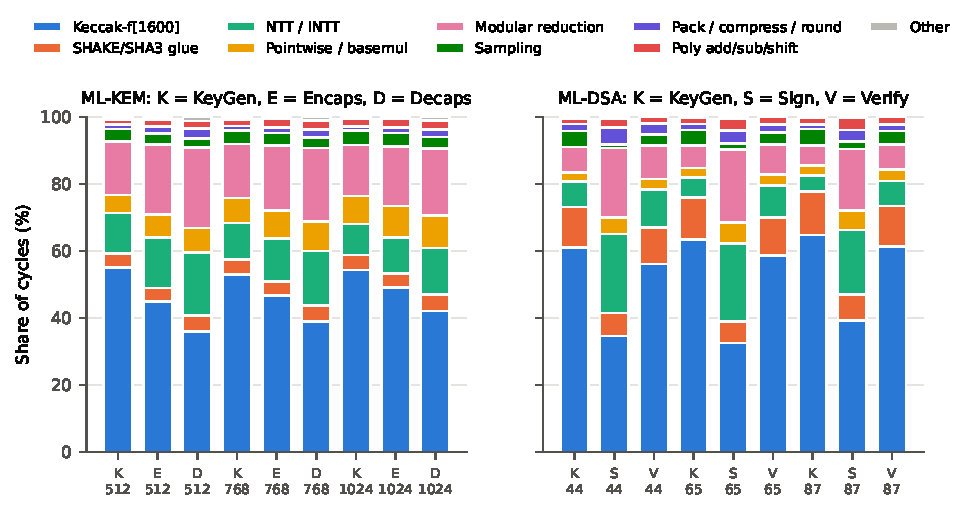
\includegraphics[width=\linewidth]{../figures/fig2_cycle_profile.pdf}\caption{\AW{caption}}\label{fig:profile}\end{figure}
\AW{Discussion of Table~\ref{tab:base} and Fig.~\ref{fig:profile}.}
\begin{facts}
\item Keccak-f[1600] share (C1-TB5): ML-KEM \FactKeccakShareKemMin--\FactKeccakShareKemMax\,\%, ML-DSA \FactKeccakShareDsaMin--\FactKeccakShareDsaMax\,\%; matches pqm4 hashing share for clean ML-KEM on M4 (32.5--50.0\,\%) \citep{pqm4}.
\item ML-DSA Sign averaged over 10 messages (rejection loop makes Sign time message-dependent; public randomness).
\end{facts}

\subsection{Microarchitecture design-space exploration}
\begin{figure}[t]\centering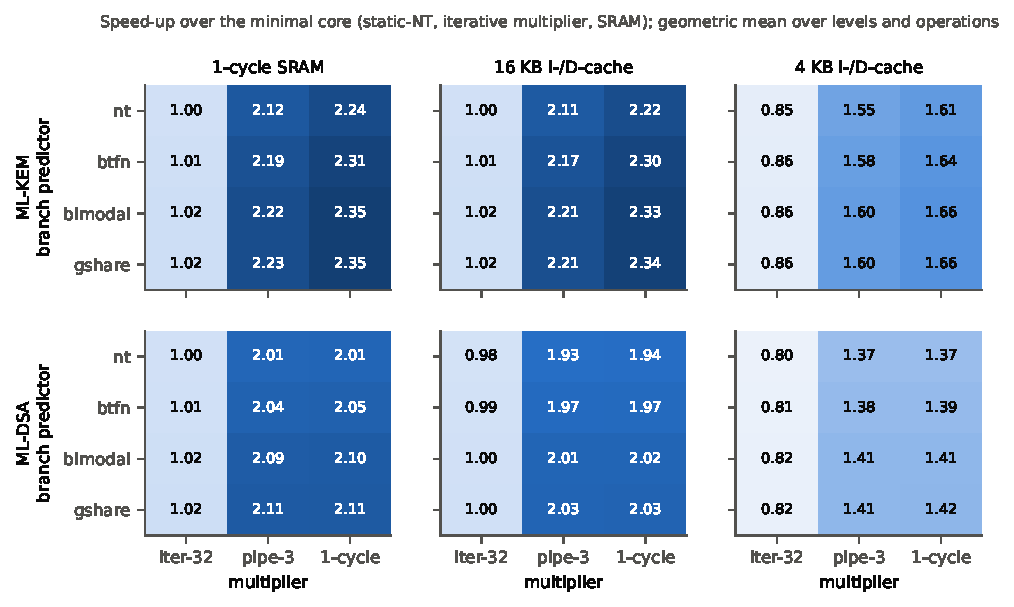
\includegraphics[width=\linewidth]{../figures/fig3_dse_heatmap.pdf}\caption{\AW{caption}}\label{fig:dse}\end{figure}
\AW{Discussion.}
\begin{facts}
\item Single-cycle vs iterative multiplier (SRAM, static NT): \FactMulGainKem$\times$ ML-KEM, \FactMulGainDsa$\times$ ML-DSA. Pipelined 3-cycle multiplier keeps most of the gain for ML-DSA, less for ML-KEM.
\item Best dynamic predictor vs static NT: only \FactBpGainKem$\times$ (ML-KEM), \FactBpGainDsa$\times$ (ML-DSA): PQC kernels are loop-dominated with regular control flow.
\item 4\,KB caches cost \FactCFourLossKem\,\% (ML-KEM) and \FactCFourLossDsa\,\% (ML-DSA) vs SRAM; 16\,KB caches are within \FactCSixteenLoss\,\%.
\end{facts}
\begin{figure}[t]\centering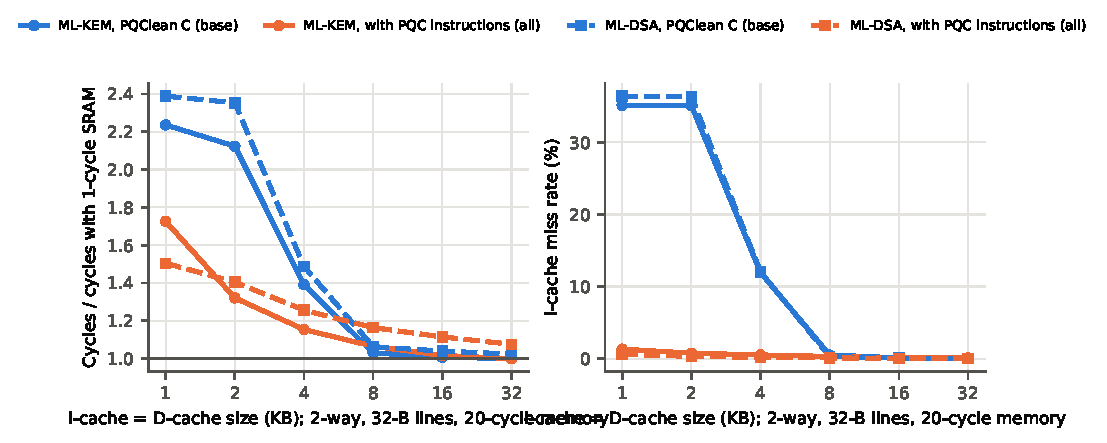
\includegraphics[width=\linewidth]{../figures/fig4_cache_sensitivity.pdf}\caption{\AW{caption}}\label{fig:cache}\end{figure}
\begin{facts}
\item Base code: I-cache miss rate \FactIcMissBaseTwo\,\% at 2\,KB, falls below 1\,\% only at \FactIcNeedBase\,KB (unrolled Keccak-f[1600] code). With the custom instructions: \FactIcMissAllOne\,\% at 1\,KB.
\item Design implication: the Keccak instruction also lets a core use a smaller I-cache, which partly pays for its area.
\end{facts}

\subsection{ISA extensions}
\begin{figure}[t]\centering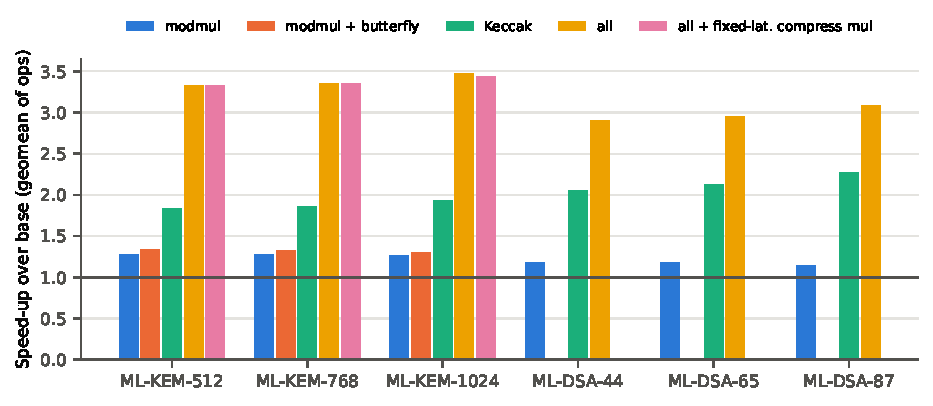
\includegraphics[width=\linewidth]{../figures/fig5_extension_speedup.pdf}\caption{\AW{caption}}\label{fig:ext}\end{figure}
\begin{figure}[t]\centering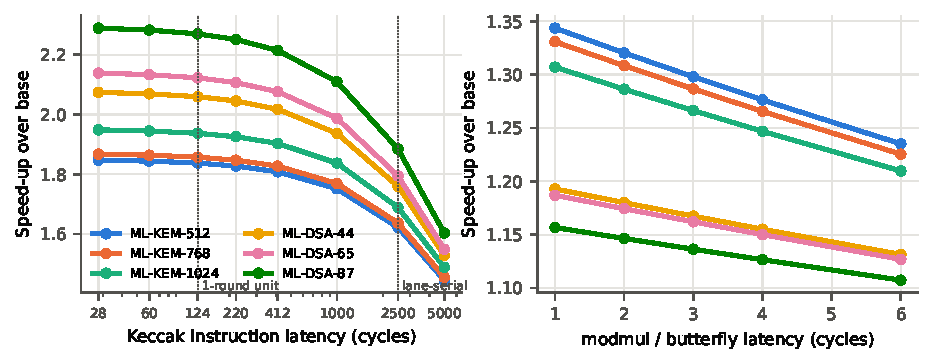
\includegraphics[width=\linewidth]{../figures/fig6_unit_latency.pdf}\caption{\AW{caption}}\label{fig:lat}\end{figure}
\begin{figure}[t]\centering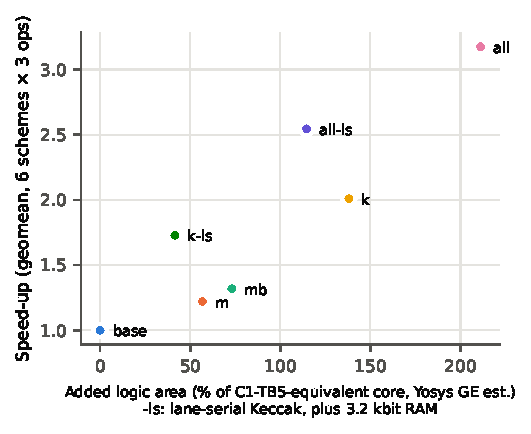
\includegraphics[width=0.6\linewidth]{../figures/fig8_area_speedup.pdf}\caption{\AW{caption}}\label{fig:area}\end{figure}
\begin{table}[t]\centering\caption{Synthesised area (Yosys generic flow). \AW{caption}}\label{tab:area}\resizebox{\linewidth}{!}{\begin{tabular}{lrrrr}\toprule
Block & GE logic (est.) & Flip-flops & LUT4 & RAM bits \\\midrule
pq.kmul/kmred/kbar (ML-KEM modmul) & 4,604 & 0 & 1,378 & 0 \\
pq.kct/kgs (ML-KEM packed butterfly) & 5,016 & 0 & 1,584 & 0 \\
pq.dmul (ML-DSA modmul) & 12,806 & 0 & 4,215 & 0 \\
pq.keccak (Keccak-f[1600], 1 round/cycle) & 42,374 & 1,613 & 9,339 & 0 \\
pq.keccak-ls (lane-serial, state in 2x25x64-bit RAM) & 12,730 & 656 & 3,959 & 3,200 \\
RV32M 32x32 single-cycle multiplier (reference) & 10,611 & 0 & 3,310 & 0 \\
Baseline RV32IM 5-stage core (author's FPGA core, no imem/dmem) & 20,070 & 1,630 & 4,045 & 0 \\
\bottomrule
\end{tabular}
}\end{table}
\begin{table}[t]\centering\caption{Division instructions executed per ML-KEM run, by compiler. \AW{caption}}\label{tab:comp}\begin{tabular}{lllrrr}\toprule
Source & Compiler & Opt. & ML-KEM-512 & ML-KEM-768 & ML-KEM-1024 \\\midrule
PQClean (current) & clang & -O2 & 0 & 0 & 0 \\
PQClean (current) & clang & -Os & 0 & 0 & 0 \\
PQClean (current) & gcc & -O2 & 56 & 80 & 104 \\
PQClean (current) & gcc & -Os & 56 & 80 & 104 \\
pre-2024 (/ q in C) & clang & -O2 & 0 & 0 & 0 \\
pre-2024 (/ q in C) & clang & -Os & 0 & 0 & 0 \\
pre-2024 (/ q in C) & gcc & -O2 & 3640 & 4688 & 5736 \\
pre-2024 (/ q in C) & gcc & -Os & 3640 & 4688 & 5736 \\
\bottomrule
\end{tabular}
\end{table}
\AW{Discussion.}
\begin{facts}
\item Speed-ups on C1-TB5 (geomean of ops): see \texttt{tables/ext\_speedup\_C1.csv}. All instructions: \FactAllSpeedMin--\FactAllSpeedMax$\times$; Keccak only: \FactKSpeedMin--\FactKSpeedMax$\times$; modmul only: \FactMSpeedMin--\FactMSpeedMax$\times$.
\item Keccak latency sweep 28$\rightarrow$412 cycles: speed-up of the Keccak-only variant falls from \FactKLatFast$\times$ to \FactKLatSlow$\times$ (geomean); a slow lane-serial unit still gives a speed-up.
\item Area (Yosys generic flow, NAND2-equivalent weights, approximate; Table~\ref{tab:area}): ML-KEM modmul unit 4.6\,kGE, packed butterfly 5.0\,kGE, ML-DSA modmul 12.8\,kGE, Keccak 1-round/cycle unit 42.4\,kGE (1613 FFs). Baseline = author's RV32IM 5-stage core 20.1\,kGE + single-cycle RV32M multiplier 10.6\,kGE = 30.7\,kGE (close to Ibex maxperf, 32.48\,kGE \citep{ibex}). All units = \FactAllAreaPct\,\% of that core (standalone units, no sharing; upper bound).
\item Keccak latency sweep 28$\rightarrow$5000 cycles: Keccak-only speed-up \FactKLatFast$\times$ $\rightarrow$ \FactKLatSlow$\times$ (geomean); flat up to $\sim$400 cycles.
\item Lane-serial Keccak unit (RTL-verified, 2500-cycle instruction): \FactLsGE\,GE logic + 3.2\,kbit RAM vs \FactKfGE\,GE for the one-round-per-cycle unit; keeps \FactKLsSpeed$\times$ (Keccak only) and \FactAllLsSpeed$\times$ (all) vs \FactKSpeedGm$\times$ and \FactAllSpeedGm$\times$.
\item The Keccak instruction also removes the need for an 8\,KB I-cache (Fig.~\ref{fig:cache}); this I-cache saving partly offsets its area \CK{SRAM area per KB depends on the technology}.
\item Compilers (Table~\ref{tab:comp}): pre-2024 C code with \texttt{/KYBER\_Q}: clang 18 emits 0 divisions (-O2 and -Os); gcc 13 emits \FactGccDivPrefix{} division instructions per ML-KEM-768 KeyGen+Encaps+Decaps (both -O2 and -Os). Current PQClean code with gcc: only \FactGccDivBase{} divisions, all in SHAKE length arithmetic (public).
\item gcc 13 -O2 code is \FactGccSlow$\times$ slower than clang 18 -O2 for base code on C1-TB5 (geomean); with all ISEs gcc reaches \FactGccAllSpeed$\times$ over clang base.
\end{facts}

\subsection{Timing leakage as a microarchitecture property}\label{sec:leak}
\begin{figure}[t]\centering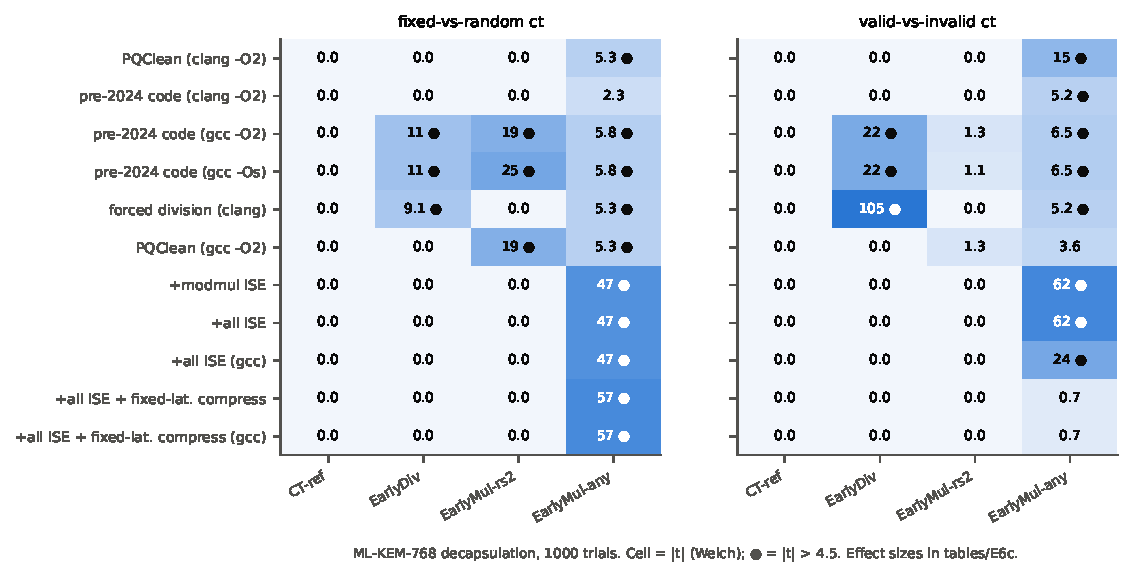
\includegraphics[width=\linewidth]{../figures/fig7_leakage.pdf}\caption{\AW{caption}}\label{fig:leak}\end{figure}
\AW{Discussion. Report effect size (cycles) next to $|t|$; deterministic simulation inflates $|t|$.}
\begin{facts}
\item Main matrix: ML-KEM-768, 1000 trials per run, with effect sizes (mean difference in cycles, Cohen's $d$) -- \texttt{E6c}; all three levels at 400 trials -- \texttt{E6}.
\item Method: ML-KEM decapsulation, 400/1000 trials per run, TVLA Welch $t$, threshold $|t|>4.5$; class applied with a branch-free masked select so pre-measurement cache/predictor state is class-independent. Tests: fixed-vs-random valid ciphertext; random valid vs random invalid ciphertext (FO implicit rejection).
\item CT-ref (1-cycle mul, fixed divider) and BP+Cache (bimodal + 8\,KB caches): zero timing variation for every variant -- PQClean branches and memory addresses are input-independent.
\item EarlyDiv: only the KyberSlash-style \texttt{kslash} variant leaks (division in \texttt{poly\_tomsg}); reproduces \citep{kyberslash2025} in simulation.
\item EarlyMul-rs2 (ARM7TDMI-style, terminates on rs2): no input-dependent latency for any clang build -- clang places the constant operand (q, QINV, zeta, 80635) in rs2 of every secret-dependent multiply. The same source built with gcc 13 leaks on this hardware (fixed-vs-random ct, $|t|\approx19$; E6b localises it to \texttt{basemul}, where gcc puts the secret operand in rs2). Leakage on such cores therefore depends on the compiler's operand order.
\item Pre-2024 reference code (\texttt{/KYBER\_Q} in C) leaks on EarlyDiv only when built with gcc ($|t|\approx11$/22), because only gcc emits the division (Table~\ref{tab:comp}); this reproduces KyberSlash from source code in simulation.
\item EarlyMul-any (terminates on the smaller operand): leaks in base, m and all. The modmul/butterfly instructions remove the NTT/basemul/reduce sources, but compress and \texttt{poly\_tomsg} remain (Table~\ref{tab:loc}). Only \texttt{allz} (constant multiplies on fixed-latency \texttt{pq.cmul}) removes the secret-dependent sources; the remaining source is \texttt{polyvec\_decompress} on the public ciphertext, which fixed-vs-random-ct flags but valid-vs-invalid does not.
\item E6c fixed-vs-random ct: \texttt{base} on \texttt{EarlyMul-any}: $|t|$=5.34, $\Delta$mean=-32.55 cycles, $d$=-0.335, spread 833 cycles.
\item E6c valid-vs-invalid ct: \texttt{base} on \texttt{EarlyMul-any}: $|t|$=15.0, $\Delta$mean=136.57 cycles, $d$=0.948, spread 929 cycles.
\item E6c fixed-vs-random ct: \texttt{kslash} on \texttt{EarlyDiv}: $|t|$=9.11, $\Delta$mean=3.81 cycles, $d$=0.571, spread 60 cycles.
\item E6c fixed-vs-random ct: \texttt{kslash} on \texttt{EarlyMul-any}: $|t|$=5.26, $\Delta$mean=-31.93 cycles, $d$=-0.33, spread 821 cycles.
\item E6c valid-vs-invalid ct: \texttt{kslash} on \texttt{EarlyDiv}: $|t|$=105.27, $\Delta$mean=-61.22 cycles, $d$=-6.651, spread 113 cycles.
\item E6c valid-vs-invalid ct: \texttt{kslash} on \texttt{EarlyMul-any}: $|t|$=5.22, $\Delta$mean=47.42 cycles, $d$=0.33, spread 888 cycles.
\item E6c fixed-vs-random ct: \texttt{m} on \texttt{EarlyMul-any}: $|t|$=46.64, $\Delta$mean=-45.7 cycles, $d$=-2.923, spread 135 cycles.
\item E6c valid-vs-invalid ct: \texttt{m} on \texttt{EarlyMul-any}: $|t|$=61.58, $\Delta$mean=88.88 cycles, $d$=3.887, spread 222 cycles.
\item E6c fixed-vs-random ct: \texttt{all} on \texttt{EarlyMul-any}: $|t|$=46.64, $\Delta$mean=-45.7 cycles, $d$=-2.923, spread 135 cycles.
\item E6c valid-vs-invalid ct: \texttt{all} on \texttt{EarlyMul-any}: $|t|$=61.58, $\Delta$mean=88.88 cycles, $d$=3.887, spread 222 cycles.
\item E6c fixed-vs-random ct: \texttt{allz} on \texttt{EarlyMul-any}: $|t|$=56.67, $\Delta$mean=-29.37 cycles, $d$=-3.552, spread 73 cycles.
\item E6c valid-vs-invalid ct: \texttt{prefix} on \texttt{EarlyMul-any}: $|t|$=5.2, $\Delta$mean=46.73 cycles, $d$=0.329, spread 866 cycles.
\item E6c fixed-vs-random ct: \texttt{prefix-gccO2} on \texttt{EarlyDiv}: $|t|$=10.77, $\Delta$mean=-20.82 cycles, $d$=-0.675, spread 281 cycles.
\item E6c fixed-vs-random ct: \texttt{prefix-gccO2} on \texttt{EarlyMul-rs2}: $|t|$=18.8, $\Delta$mean=-71.93 cycles, $d$=-1.179, spread 494 cycles.
\item E6c fixed-vs-random ct: \texttt{prefix-gccO2} on \texttt{EarlyMul-any}: $|t|$=5.75, $\Delta$mean=-27.66 cycles, $d$=-0.36, spread 651 cycles.
\item E6c valid-vs-invalid ct: \texttt{prefix-gccO2} on \texttt{EarlyDiv}: $|t|$=21.91, $\Delta$mean=-63.39 cycles, $d$=-1.385, spread 325 cycles.
\item E6c valid-vs-invalid ct: \texttt{prefix-gccO2} on \texttt{EarlyMul-any}: $|t|$=6.51, $\Delta$mean=45.11 cycles, $d$=0.412, spread 652 cycles.
\item E6c fixed-vs-random ct: \texttt{prefix-gccOs} on \texttt{EarlyDiv}: $|t|$=10.77, $\Delta$mean=-20.82 cycles, $d$=-0.675, spread 281 cycles.
\item E6c fixed-vs-random ct: \texttt{prefix-gccOs} on \texttt{EarlyMul-rs2}: $|t|$=24.9, $\Delta$mean=-98.18 cycles, $d$=-1.561, spread 544 cycles.
\item E6c fixed-vs-random ct: \texttt{prefix-gccOs} on \texttt{EarlyMul-any}: $|t|$=5.75, $\Delta$mean=-27.66 cycles, $d$=-0.36, spread 651 cycles.
\item E6c valid-vs-invalid ct: \texttt{prefix-gccOs} on \texttt{EarlyDiv}: $|t|$=21.91, $\Delta$mean=-63.39 cycles, $d$=-1.385, spread 325 cycles.
\item E6c valid-vs-invalid ct: \texttt{prefix-gccOs} on \texttt{EarlyMul-any}: $|t|$=6.51, $\Delta$mean=45.11 cycles, $d$=0.412, spread 652 cycles.
\item E6c fixed-vs-random ct: \texttt{base-gccO2} on \texttt{EarlyMul-rs2}: $|t|$=18.8, $\Delta$mean=-71.93 cycles, $d$=-1.179, spread 494 cycles.
\item E6c fixed-vs-random ct: \texttt{base-gccO2} on \texttt{EarlyMul-any}: $|t|$=5.26, $\Delta$mean=-25.39 cycles, $d$=-0.33, spread 654 cycles.
\item E6c fixed-vs-random ct: \texttt{all-gccO2} on \texttt{EarlyMul-any}: $|t|$=47.26, $\Delta$mean=-27.09 cycles, $d$=-2.962, spread 79 cycles.
\item E6c valid-vs-invalid ct: \texttt{all-gccO2} on \texttt{EarlyMul-any}: $|t|$=23.94, $\Delta$mean=-20.62 cycles, $d$=-1.514, spread 100 cycles.
\item E6c fixed-vs-random ct: \texttt{allz-gccO2} on \texttt{EarlyMul-any}: $|t|$=56.67, $\Delta$mean=-29.37 cycles, $d$=-3.552, spread 73 cycles.
\item E6c: 27 of 44 (code, hardware) pairs show no leak in either test.

\item Hypothesis from the literature review (``fixed-latency PQC instructions remove multiplier leakage'') is only partly true -- confirmed by data.
\item fixed-vs-random ct: LEAK for variant \texttt{all} on \texttt{All-variable} (ml-kem-1024,ml-kem-512,ml-kem-768); max $|t|$=30.6, max spread 149 cycles.
\item fixed-vs-random ct: LEAK for variant \texttt{all} on \texttt{EarlyMul-any} (ml-kem-1024,ml-kem-512,ml-kem-768); max $|t|$=30.6, max spread 149 cycles.
\item fixed-vs-random ct: LEAK for variant \texttt{allz} on \texttt{All-variable} (ml-kem-1024,ml-kem-768); max $|t|$=34.9, max spread 73 cycles.
\item fixed-vs-random ct: LEAK for variant \texttt{allz} on \texttt{EarlyMul-any} (ml-kem-1024,ml-kem-768); max $|t|$=34.9, max spread 73 cycles.
\item fixed-vs-random ct: LEAK for variant \texttt{base} on \texttt{All-variable} (ml-kem-1024,ml-kem-512); max $|t|$=15.2, max spread 1091 cycles.
\item fixed-vs-random ct: LEAK for variant \texttt{base} on \texttt{EarlyMul-any} (ml-kem-1024,ml-kem-512); max $|t|$=15.2, max spread 1091 cycles.
\item fixed-vs-random ct: LEAK for variant \texttt{kslash} on \texttt{All-variable} (ml-kem-1024,ml-kem-512); max $|t|$=14.2, max spread 1089 cycles.
\item fixed-vs-random ct: LEAK for variant \texttt{kslash} on \texttt{EarlyDiv} (ml-kem-1024,ml-kem-512,ml-kem-768); max $|t|$=10.3, max spread 60 cycles.
\item fixed-vs-random ct: LEAK for variant \texttt{kslash} on \texttt{EarlyMul-any} (ml-kem-1024,ml-kem-512); max $|t|$=15.3, max spread 1085 cycles.
\item fixed-vs-random ct: LEAK for variant \texttt{m} on \texttt{All-variable} (ml-kem-1024,ml-kem-512,ml-kem-768); max $|t|$=30.6, max spread 149 cycles.
\item fixed-vs-random ct: LEAK for variant \texttt{m} on \texttt{EarlyMul-any} (ml-kem-1024,ml-kem-512,ml-kem-768); max $|t|$=30.6, max spread 149 cycles.
\item fixed-vs-random ct: 19 of 30 (variant, hardware) pairs show no leak at $|t|\le4.5$ for all three ML-KEM levels.
\item valid-vs-invalid ct: LEAK for variant \texttt{all} on \texttt{All-variable} (ml-kem-1024,ml-kem-512,ml-kem-768); max $|t|$=45.1, max spread 218 cycles.
\item valid-vs-invalid ct: LEAK for variant \texttt{all} on \texttt{EarlyMul-any} (ml-kem-1024,ml-kem-512,ml-kem-768); max $|t|$=45.3, max spread 218 cycles.
\item valid-vs-invalid ct: LEAK for variant \texttt{base} on \texttt{All-variable} (ml-kem-1024,ml-kem-512,ml-kem-768); max $|t|$=13.8, max spread 1168 cycles.
\item valid-vs-invalid ct: LEAK for variant \texttt{base} on \texttt{EarlyMul-any} (ml-kem-1024,ml-kem-512,ml-kem-768); max $|t|$=13.8, max spread 1168 cycles.
\item valid-vs-invalid ct: LEAK for variant \texttt{kslash} on \texttt{EarlyDiv} (ml-kem-1024,ml-kem-512,ml-kem-768); max $|t|$=77.2, max spread 118 cycles.
\item valid-vs-invalid ct: LEAK for variant \texttt{kslash} on \texttt{EarlyMul-any} (ml-kem-512); max $|t|$=5.5, max spread 772 cycles.
\item valid-vs-invalid ct: LEAK for variant \texttt{m} on \texttt{All-variable} (ml-kem-1024,ml-kem-512,ml-kem-768); max $|t|$=45.3, max spread 218 cycles.
\item valid-vs-invalid ct: LEAK for variant \texttt{m} on \texttt{EarlyMul-any} (ml-kem-1024,ml-kem-512,ml-kem-768); max $|t|$=45.3, max spread 218 cycles.
\item valid-vs-invalid ct: 22 of 30 (variant, hardware) pairs show no leak at $|t|\le4.5$ for all three ML-KEM levels.

\end{facts}
\begin{table}[t]\centering\caption{Instructions whose latency depends on the decapsulation input (ML-KEM-768). Operand class assigned by function \CK{manual classification}. \AW{caption}}\label{tab:loc}
\resizebox{\linewidth}{!}{\begin{tabular}{lllrl}\toprule
Hardware & Variant & Function & \#input-dep.\ instr. & Operand data \\\midrule
EarlyMul-any & base & barrett\_reduce & 1 & secret-derived \\
EarlyMul-any & base & basemul & 5 & secret-derived \\
EarlyMul-any & base & invntt & 2 & secret-derived \\
EarlyMul-any & base & montgomery\_reduce & 2 & secret-derived \\
EarlyMul-any & base & ntt & 1 & secret-derived \\
EarlyMul-any & base & poly\_compress & 8 & secret-derived \\
EarlyMul-any & base & poly\_tomsg & 8 & secret-derived \\
EarlyMul-any & base & polyvec\_compress & 8 & secret-derived \\
EarlyMul-any & base & polyvec\_decompress & 4 & public (ciphertext u) \\
EarlyDiv & kslash & poly\_tomsg & 8 & secret-derived \\
EarlyMul-any & kslash & barrett\_reduce & 1 & secret-derived \\
EarlyMul-any & kslash & basemul & 5 & secret-derived \\
EarlyMul-any & kslash & invntt & 2 & secret-derived \\
EarlyMul-any & kslash & montgomery\_reduce & 2 & secret-derived \\
EarlyMul-any & kslash & ntt & 1 & secret-derived \\
EarlyMul-any & kslash & poly\_compress & 8 & secret-derived \\
EarlyMul-any & kslash & polyvec\_compress & 8 & secret-derived \\
EarlyMul-any & kslash & polyvec\_decompress & 4 & public (ciphertext u) \\
EarlyMul-any & m & poly\_compress & 8 & secret-derived \\
EarlyMul-any & m & poly\_tomsg & 8 & secret-derived \\
EarlyMul-any & m & polyvec\_compress & 8 & secret-derived \\
EarlyMul-any & m & polyvec\_decompress & 4 & public (ciphertext u) \\
EarlyMul-any & all & poly\_compress & 8 & secret-derived \\
EarlyMul-any & all & poly\_tomsg & 8 & secret-derived \\
EarlyMul-any & all & polyvec\_compress & 8 & secret-derived \\
EarlyMul-any & all & polyvec\_decompress & 4 & public (ciphertext u) \\
EarlyMul-any & allz & polyvec\_decompress & 4 & public (ciphertext u) \\
EarlyMul-any & prefix & barrett\_reduce & 1 & secret-derived \\
EarlyMul-any & prefix & basemul & 5 & secret-derived \\
EarlyMul-any & prefix & invntt & 2 & secret-derived \\
EarlyMul-any & prefix & montgomery\_reduce & 2 & secret-derived \\
EarlyMul-any & prefix & ntt & 1 & secret-derived \\
EarlyMul-any & prefix & polyvec\_compress & 4 & secret-derived \\
EarlyMul-any & prefix & polyvec\_decompress & 4 & public (ciphertext u) \\
EarlyDiv & prefix-gccO2 & poly\_compress & 1 & secret-derived \\
EarlyDiv & prefix-gccO2 & poly\_tomsg & 1 & secret-derived \\
EarlyDiv & prefix-gccO2 & polyvec\_compress & 1 & secret-derived \\
EarlyMul-rs2 & prefix-gccO2 & basemul & 4 & secret-derived \\
EarlyMul-any & prefix-gccO2 & barrett\_reduce & 1 & secret-derived \\
EarlyMul-any & prefix-gccO2 & basemul & 5 & secret-derived \\
EarlyMul-any & prefix-gccO2 & invntt & 2 & secret-derived \\
EarlyMul-any & prefix-gccO2 & montgomery\_reduce & 2 & secret-derived \\
EarlyMul-any & prefix-gccO2 & ntt & 1 & secret-derived \\
EarlyMul-any & prefix-gccO2 & polyvec\_decompress & 1 & public (ciphertext u) \\
EarlyDiv & prefix-gccOs & poly\_compress & 1 & secret-derived \\
EarlyDiv & prefix-gccOs & poly\_tomsg & 1 & secret-derived \\
EarlyDiv & prefix-gccOs & polyvec\_compress & 1 & secret-derived \\
EarlyMul-rs2 & prefix-gccOs & basemul & 4 & secret-derived \\
EarlyMul-rs2 & prefix-gccOs & invntt & 1 & secret-derived \\
EarlyMul-any & prefix-gccOs & barrett\_reduce & 1 & secret-derived \\
EarlyMul-any & prefix-gccOs & basemul & 5 & secret-derived \\
EarlyMul-any & prefix-gccOs & invntt & 2 & secret-derived \\
EarlyMul-any & prefix-gccOs & montgomery\_reduce & 2 & secret-derived \\
EarlyMul-any & prefix-gccOs & ntt & 1 & secret-derived \\
EarlyMul-any & prefix-gccOs & polyvec\_decompress & 1 & public (ciphertext u) \\
EarlyMul-rs2 & base-gccO2 & basemul & 4 & secret-derived \\
EarlyMul-any & base-gccO2 & barrett\_reduce & 1 & secret-derived \\
EarlyMul-any & base-gccO2 & basemul & 5 & secret-derived \\
EarlyMul-any & base-gccO2 & invntt & 2 & secret-derived \\
EarlyMul-any & base-gccO2 & montgomery\_reduce & 2 & secret-derived \\
EarlyMul-any & base-gccO2 & ntt & 1 & secret-derived \\
EarlyMul-any & base-gccO2 & polyvec\_compress & 1 & secret-derived \\
EarlyMul-any & base-gccO2 & polyvec\_decompress & 1 & public (ciphertext u) \\
EarlyMul-any & all-gccO2 & polyvec\_compress & 1 & secret-derived \\
EarlyMul-any & all-gccO2 & polyvec\_decompress & 1 & public (ciphertext u) \\
EarlyMul-any & allz-gccO2 & polyvec\_decompress & 1 & public (ciphertext u) \\
\bottomrule
\end{tabular}
}\end{table}

%% =====================================================================
\section{Discussion}\label{sec:disc}
\AW{Design guidelines for embedded PQC cores; threats to validity (timing model validated against one RTL core, other cores via parameters; area from a generic Yosys flow, not a PDK or Quartus; no physical power/EM channels; deterministic $t$-test inflates $|t|$, hence effect sizes); how to extend to FPGA board measurements.}

\section{Conclusion}\label{sec:concl}
\AW{Conclusion.}

\section*{Data availability}
\AW{GitHub URL and Zenodo DOI of the PQ-uArch repository.}

\section*{Declaration of generative AI use}
\AW{Elsevier requires a statement if AI tools were used (e.g., for code). Write it per the Guide for Authors.} \CK{check JSA policy text}

\bibliographystyle{elsarticle-harv}
\bibliography{references}
\end{document}
